
\section{\trZariski{}连通性引理与\trStein{}因子分解}

我们现在来陈述并证明\trZariski{}连通性引理，它曾在 \S25.1.8 中被提及。

\textbf{28.4.1. \trZariski{}连通性引理。}\ ——\ \emph{若局部\trNoether{}\trScheme{}之间的一个\trProper\trMorphism{} $\pi\colon X\to Y$ 是 $\OO$-连通的（见 \S25.1.7），则对每个 $q\in Y$，$\pi^{-1}(q)$ 都是\trConnected{}的。}

该证明需要下面的结果。

\textbf{28.4.A.（容易练习：局部环的完备化是局部环）}\quad 设 $(A,\mathfrak{m})$ 是一个\trNoetherian\trLocalRing。证明：$A$ 沿 $\mathfrak{m}$ 的\trCompletion，即 $\hat{A}:=\lim A/\mathfrak{m}^n$，是一个\trLocalRing，其\trMaximalIdeal{}为 $\mathfrak{m}\hat{A}$。提示：证明 $\hat{A}$ 中任何不属于 $\mathfrak{m}\hat{A}$ 的元素都\trInvertible。

\emph{证明。}\quad 假设不然：存在某个 $q\in Y$ 使得 $\pi^{-1}(q)$ 不\trConnected，比方说 $\pi^{-1}(q)=X_1\coprod X_2$（其中 $X_1$ 与 $X_2$ 是这条\trFiber{}的两个非空\trOpenSubset；见\cref{fig:formal-neighborhoods}）。于是 $\pi^{-1}(q)$ 的 $n$ 阶形式邻域，由于带有同一个\trTopologicalSpace，也是不\trConnected{}的。我们使用\trIdempotent{}这一实用技巧（\mbox{注记~3.6.3}）。令 $e_1$ 为在 $X_1$ 上取值 $1$、在 $X_2$ 上取值 $0$ 的函数，并令 $e_2$ 为在 $X_2$ 上取值 $1$、在 $X_1$ 上取值 $0$ 的函数。这些函数在任何阶的形式邻域上都有意义，而且它们在\trInverseLimit{}中有自然的像。由\mbox{形式函数定理~28.3.2} 给出的\trIsomorphism（施用于 $\mathrm{H}^0$），我们得到 $\hat{\OO}_{Y,q}$ 中的非零元 $e_1$ 与 $e_2$，满足 $e_1+e_2=1$、$e_1e_2=0$。此时，$\hat{\OO}_{Y,q}$ 是一个\trLocalRing（\mbox{练习~28.4.A}）。但 $e_1e_2=0$ 蕴含 $e_1$ 与 $e_2$ 都不\trInvertible（否则另一个就会是 $0$），于是 $e_1$ 与 $e_2$ 都落在\trMaximalIdeal{}中，从而 $e_1+e_2$ 不可能是 $1$。我们由此得到矛盾。\hfill$\square$

\begin{figure}[htbp]
\centering
\begin{tikzpicture}[x=1cm,y=1cm,>=stealth,line width=0.5pt]
\node (X1) at (1.45,0.75)  {$X_1$};
\node (X2) at (1.55,0.05)  {$X_2$};
\draw[->,densely dashed] (0.55,0.75) -- (1.05,0.75);
\draw[->,densely dashed] (0.65,0.05) -- (1.15,0.05);
\draw[->,gray!70!black!60,line width=0.9pt] (0.95,-0.5) -- (0.95,-2.25);
\node at (0.95,-2.62) {$\bullet$};
\node at (0.95,-3.0)  {$q$};
\draw[line width=0.6pt] (-1.3,-2.55) .. controls (-0.5,-2.8) and (0.1,-2.45) ..
      (0.95,-2.62) .. controls (1.8,-2.8) and (2.4,-2.5) .. (2.75,-2.4);
\node at (3.15,-2.2) {$Y$};
\end{tikzpicture}
\caption{\mbox{\trZariski{}连通性引理~28.4.1} 证明中 $X_1$ 与 $X_2$ 的「形式邻域」。（依原书手绘图重绘。）}
\label{fig:formal-neighborhoods}
\end{figure}

\textbf{28.4.2. \trStein{}因子分解。}\quad 我们接下来描述那个被称为「\trStein{}因子分解」（Stein factorization）的构造。我们本可以早早地就把它定义出来，但现在，\mbox{\trZariski{}连通性引理~28.4.1} 将给我们带来一些令人瞩目的推论。

\textbf{28.4.3. \trStein{}因子分解定理。}\ ——\ \emph{任何局部\trNoether{}\trScheme{}之间的\trProper\trMorphism{} $\pi\colon X\to Y$ 都可以分解为 $\beta\circ\alpha$，其中 $\alpha\colon X\to Y'$ 是\trProper{}且 $\OO$-连通的（从而由\mbox{\trZariski{}连通性引理~28.4.1}，它具有\trConnected{}的\trFiber），而 $\beta\colon Y'\to Y$ 是一个\trFinite\trMorphism。}

\begin{equation*}
\tag{28.4.3.1}\label{eq:stein-factorization-triangle}
\begin{tikzcd}[row sep=2.8em, column sep=4.5em]
X \ar[rr, "\text{$\OO$-conn.}", "\alpha"'] \ar[dr, "\pi"'] && {Y'} \ar[dl, "\beta", "\text{finite}"'] \\
& Y &
\end{tikzcd}
\end{equation*}

我们指出：由\trProjective\trMorphism{}的消去定理（\mbox{练习~17.3.C}），若 $\pi$ 恰好是\trProjective{}的，那么 $\alpha$ 也是（因为 $\delta_\beta$ 作为\trClosedEmbedding{}是\trProjective{}的）。

尽管定理的陈述并未把它说出来，但证明实际上给出了一个\emph{特定的}因子分解，它被称为 $\pi$ 的\textbf{\trStein{}因子分解}。你心中应有的图景是：\trStein{}因子分解（大体上）以某种典范的方式把\trFiber{}的连续部分\footnote{原书此处作「continuous parts」，疑当为「connected parts」（连通部分），兹照录原书。——译者注}收缩掉；见\cref{fig:stein-factorization}。

\begin{figure}[htbp]
\centering
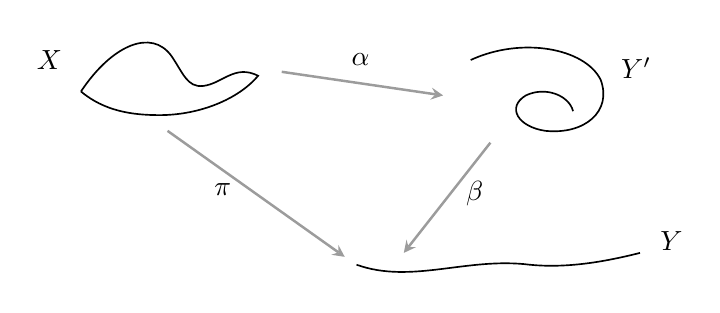
\begin{tikzpicture}[x=1cm,y=1cm,>=stealth,line width=0.5pt]
\draw[line width=0.6pt] (-0.6,0.55) .. controls (-0.2,1.15) and (0.3,1.35) .. (0.55,1.0)
      .. controls (0.7,0.78) and (0.75,0.6) .. (0.95,0.62)
      .. controls (1.2,0.65) and (1.35,0.9) .. (1.65,0.75)
      .. controls (1.4,0.45) and (0.9,0.25) .. (0.4,0.25)
      .. controls (0.05,0.25) and (-0.3,0.3) .. (-0.6,0.55);
\node at (-1.0,0.95) {$X$};
\draw[line width=0.6pt] (4.35,0.95) .. controls (5.0,1.25) and (5.8,1.1) .. (6.0,0.7)
      .. controls (6.15,0.3) and (5.8,0.0) .. (5.3,0.05)
      .. controls (4.95,0.1) and (4.8,0.35) .. (5.05,0.5)
      .. controls (5.3,0.62) and (5.6,0.5) .. (5.65,0.3);
\node at (6.45,0.85) {$Y'$};
\draw[line width=0.6pt] (2.9,-1.65) .. controls (3.6,-1.9) and (4.3,-1.55) .. (5.1,-1.65)
      .. controls (5.6,-1.7) and (6.1,-1.6) .. (6.5,-1.5);
\node at (6.9,-1.35) {$Y$};
\draw[->,gray!70!black!60,line width=0.9pt] (1.95,0.8) -- (4.0,0.5);
\node at (2.95,0.95) {$\alpha$};
\draw[->,gray!70!black!60,line width=0.9pt] (0.5,0.05) -- (2.75,-1.55);
\node at (1.2,-0.7) {$\pi$};
\draw[->,gray!70!black!60,line width=0.9pt] (4.6,-0.1) -- (3.5,-1.5);
\node at (4.4,-0.75) {$\beta$};
\end{tikzpicture}
\caption{\trStein{}因子分解。（依原书手绘图重绘。）}
\label{fig:stein-factorization}
\end{figure}

如常，\trNoether{}假设可以去掉（见 [Stacks, tag 03H2]）。

\emph{\mbox{\trStein{}因子分解定理~28.4.3} 的证明。}\quad 由\mbox{\trGrothendieck{}凝聚定理~18.9.1}，$\pi_*\OO_X$ 是 $Y$ 上的一个\trCoherentSheaf（\trSheafOfAlgebras）。令 $Y':=\Spec\pi_*\OO_X$，于是（由于 $\pi_*\OO_X$ 是\trFiniteType{}的）\trStructureMorphism{} $\beta\colon Y'\to Y$ 是有限的。我们有一个因子分解
\[
\begin{tikzcd}[row sep=2.8em, column sep=4.5em]
X \ar[rr, "\alpha"'] \ar[dr, "\pi"'] && {Y'} \ar[dl, "\beta", "\text{finite}"'] \\
& Y &
\end{tikzcd}
\]
由针对\trProper\trMorphism{}的\mbox{\trCancellationTheorem~11.1.1}，$\alpha$ 是\trProper{}的。最后，我们证明 $\alpha$ 是 $\OO$-连通的，也就是说，$\OO_{Y'}\to\alpha_*\OO_X$ 是一个\trIsomorphism。由于 $\beta$ 是仿射\trMorphism（从而 $\beta_*$ 是从 $\mathit{Coh}_{Y'}$ 到 $\mathit{Coh}_Y$ 的一个\trExact\trFunctor），所以施以前推 $\beta_*$ 之后再作检验就足够了。但 $\beta_*\OO_{Y'}\to\beta_*\alpha_*\OO_X$ 就是恒等映射 $\pi_*\OO_X\to\pi_*\OO_X$（这里我们用到 $\beta_*\OO_{Y'}=\pi_*\OO_X$——见 \S17.1.4——以及 $\beta_*\alpha_*\OO_X=\pi_*\OO_X$）。\hfill$\square$

\textbf{28.4.B.（练习）}\quad 设 $\pi\colon X\to Y$ 是不可约\trVariety{}之间的一个\trProper{}、\trBirational{}\trMorphism。再设 $Y$ 是\trNormal{}的。证明：$\pi$ 是 $\OO$-连通的。（例如，这适用于沿光滑\trCenter{}对光滑\trVariety{}作\trBlowup{}的情形。）于是，由\mbox{\trZariski{}连通性引理~28.4.1}，$\pi$ 具有\trConnected{}的\trFiber。这被称为\mbox{\trZariskiMainTheorem}（双有理\trMorphism{}的版本）。提示：\mbox{练习~10.7.P}。

\textbf{28.4.C.（练习）}\quad 设 $\pi\colon X\to Y$ 与 $\pi'\colon X\to Y'$ 是整的局部\trNoether{}\trScheme{}之间的两个\trProper{}、\trBirational{}\trMorphism，各自把 $X$ 的同一个\trConnected{}集合收缩为一点（而在其余之处是\trIsomorphism），并设 $Y$ 与 $Y'$ 都是\trNormal{}的。证明：$\pi$ 与 $\pi'$ 是相同的\trMorphism（或更确切地说：存在\trIsomorphism{} $i\colon Y\xrightarrow{\ \sim\ }Y'$ 使得 $\pi'=i\circ\pi$）。非正式的转述：若 $X\to Y$ 具有\trConnected{}的\trFiber，那么仅凭知道 $X$ 上被收缩的\trLocus，$Y$ 就被确定了。提示：先把 $Y$ 与 $Y'$ 作为\trTopologicalSpace{}等同起来，再把 $\pi$ 与 $\pi'$ 作为\trTopologicalSpace{}之间的映射等同起来。用\trStein{}因子分解去复原作为 $\pi_*\OO_X$ 的\trStructureSheaf。

\textbf{28.4.D.（练习）}\quad 证明：局部\trNoether{}\trScheme{}之间的\trMorphism{} $\pi\colon X\to Y$ 的\trStein{}因子分解的构造，与局部\trNoether{}\trScheme{}之间的任何\trFlat\trBaseChange{} $Z\to Y$ 相交换。

\textbf{28.4.4. \trCurve{}的\trResolutionOfSingularities。}

若 $C$ 是域 $k$ 上的一条既约\trProjective\trCurve，那么我们可以通过\trNormalization{}来解消它的奇点：$\nu\colon\tilde{C}\to C$。（关于\trResolutionOfSingularities{}的一些讨论见\mbox{注记~22.4.6}；正规\trCurve{}是\trRegular{}的理由见\mbox{定理~13.5.8}。）但从诸例子中我们已经看到，想弄清如何取\trIntegralClosure{}既需要运气也需要洞察力，而我常常两者皆无。我们现在要通过解释如何用\trBlowup{}去奇点，来除掉去奇点过程中的（需要灵感的）猜测成分。算法很简单：我们找到一个\trSingularPoint，把它胀开，然后再寻找更多的\trSingularPoint{}来重复这一过程。显然，如果找不到\trSingularPoint{}了，我们就完工了；问题在于要证明这一过程保证会终止。我们靠利用一个整数不变量来做到这一点：\trArithmeticGenus。我们必须证明：(i) 若 $p_a(\tilde{C})=p_a(C)$，则 $\nu$ 是一个\trIsomorphism——$\tilde{C}$ 已经是非奇异的；(ii) 若 $C'\to C$ 是一个\trBirational\trMorphism，则 $p_a(C')\le p_a(C)$（于是 $p_a(\tilde{C})$ 将是整个过程中\trArithmeticGenus{}的一个下界）；以及 (iii) 胀开一个\trSingularPoint{}会使\trArithmeticGenus{}下降。

为建立这些结果，我们考虑如下的情境。设 $\pi\colon C'\to C$ 是一个\trFinite\trMorphism（其中 $C$ 如上一段所述，而 $C'$ 是一条既约\trCurve），它在 $C$ 的一个有限闭子集之外是\trIsomorphism（从而 $\pi$ 是\trBirational{}的）。于是，拉回映射 $\OO_C\to\pi_*\OO_{C'}$ 没有核，因为 $C$ 是既约的；而且该映射在 $C$ 的各分量的一般点处是\trIsomorphism。其余核 $\mathscr{G}$ 的\trSupport{}落在由有限个\trClosedPoint{}组成的集合上，于是对 $i>0$ 有 $\mathrm{H}^i(C,\mathscr{G})=0$；并且若 $\mathrm{H}^0(C,\mathscr{G})=0$，则 $\mathscr{G}=0$。从正合列
\[
0\longrightarrow\OO_C\longrightarrow\pi_*\OO_{C'}\longrightarrow\mathscr{G}\longrightarrow 0,
\]
以及 $\pi$ 为仿射这一事实，可得 $\chi(C',\OO_{C'})=\chi(C,\OO_C)+\chi(C,\mathscr{G})$，从而 $p_a(C)\ge p_a(C')$，而等号成立当且仅当 $\pi$ 是 $\OO$-连通的（即 $\mathscr{G}=0$）。

\textbf{28.4.E.（练习）}\quad 证明：若 $\pi$（如上）是 $\OO$-连通的，则 $\pi$ 是一个\trIsomorphism。提示：证明仿射的 $\OO$-连通\trMorphism{}都是\trIsomorphism。

为完成我们的策略，还剩一件事要证：若 $\beta\colon C'\to C$ 是 $C$ 在一点 $p$ 处的\trBlowup，而 $\beta$ 是一个\trIsomorphism，则 $C$ 在该点处已经是非奇异的。但如果 $\beta$ 是\trIsomorphism，那么 $p$ 就是\trExceptionalDivisor，从而是一个\trEffectiveCartierDivisor，从而局部地由单个方程\footnote{原书此处作「a singular equation」，按文义当为「a single equation」之误（single 误排作 singular），径改。——译者注}截出。但这样一来，$\mathfrak{m}_{C,p}\subset\OO_{C,p}$ 就是\trPrincipal{}的，故 $\OO_{C,p}$ 是一个维数为 $1$ 的\trRegular\trLocalRing。

（你应当核实一下：我们确实完成了我们的策略。你能把这个论证推广到 $C$ 非\trProjective{}的情形吗？）

曲面的\trResolutionOfSingularities{}将在 \S28.6.4 中简略讨论。
